
\section{Metodologie analizzate}\label{metodologie}

Gli algoritmi paralleli che calcolano la trasposta di una matrice sparsa descritti in \cite{parallelTrans} vengono confrontati nelle tempistiche rispetto all'algoritmo seriale e rispetto alle funzioni di libreria \cuSPARSE{} fornite da NVidia come parte della loro piattaforma Cuda SDK. 

Per convenzione la matrice è in formato \emph{csr}. I nomi delle componenti della matrice sono chiamati \var{csr\_row\_ptr} (lunghezza $\mathrm{m}+1$) per il vettore dei puntatori ad inizio riga, \var{csr\_col\_idx} (lunghezza $\mathrm{nnz}$) per il vettore degli indici di colonna e \var{csr\_val} (lunghezza $\mathrm{nnz}$) per il vettore dei valori. 
		
\subsection{Trasposta seriale}

\begin{figure}[htbp]
    \centering
	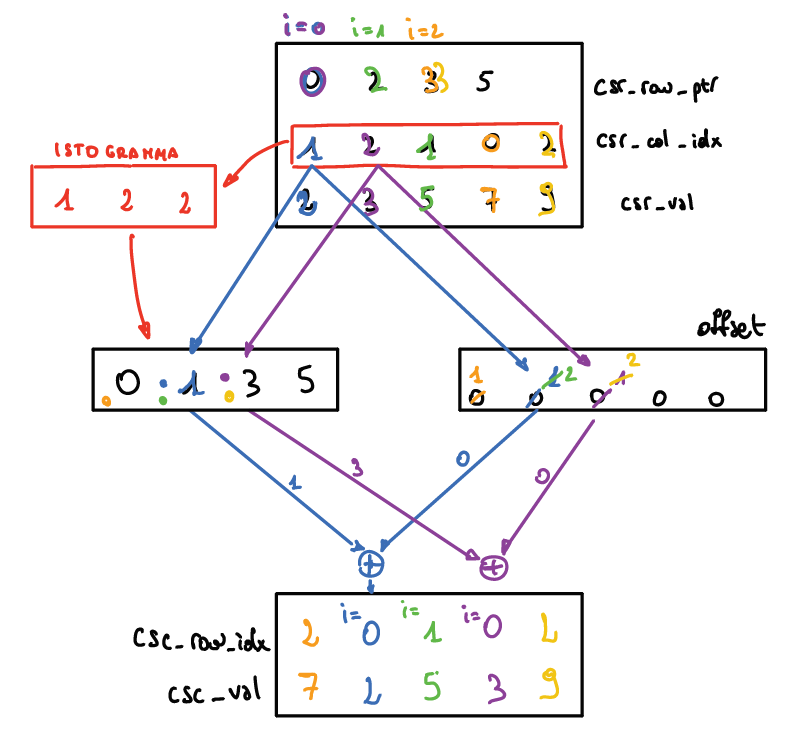
\includegraphics[scale=0.5]{transpose_algo_serial.PNG}
	\caption{Algoritmo seriale}
	\label{transpose_algo_serial}
\end{figure}

L'algoritmo si sviluppa nel seguente modo:
\begin{enumerate}
    \item si applica la funzione \emph{istogramma} \var{csr\_col\_idx} che calcola le occorrenze di ogni colonna, applicando \emph{scan} si ottiene il vettore \var{csc\_col\_ptr} (lunghezza $\mathrm{n}+1$) che conterrà i puntatori agli elementi di inizio riga trasposta;
    \item allochiamo il vettore \var{csc\_row\_idx} contente gli indici di riga (lunghezza $\mathrm{nnz}$);
    \item allochiamo il vettore \var{csc\_val} contente gli elementi non nulli (lunghezza $\mathrm{nnz}$);
    \item per ogni riga $i \in [0, m)$ processiamo gli elementi corrispondenti all'$i$-esima riga, legati alle posizioni $j \in [\var{csr\_row\_ptr}[i], \var{csr\_row\_ptr}[i+1])$
    \begin{itemize}
        \item la locazione $\mathrm{loc}$ del $j$-esimo elemento ordinata per righe è $\var{csc\_col\_ptr}[j] + \mathrm{offset}[j]$ dove $\mathrm{offset}[j]$ è un contatore incrementato ogni volta che aggiungiamo un elemento della colonna $\var{csc\_col\_ptr}[j]$;
        \item l'indice di riga dell'elemento $\mathrm{loc}$-esimo è $i$;
        % TODO mettere il nome di fianco all'array di sx?
        \item il valore dell'elemento  $\mathrm{loc}$-esimo è $\var{csr\_val}[j]$.
    \end{itemize}
\end{enumerate}

L'esecuzione dell'algoritmo seriale è illustrato in Figura~\ref{transpose_algo_serial}.

\subsection{ScanTrans}

\begin{figure}[htbp]
    \centering
	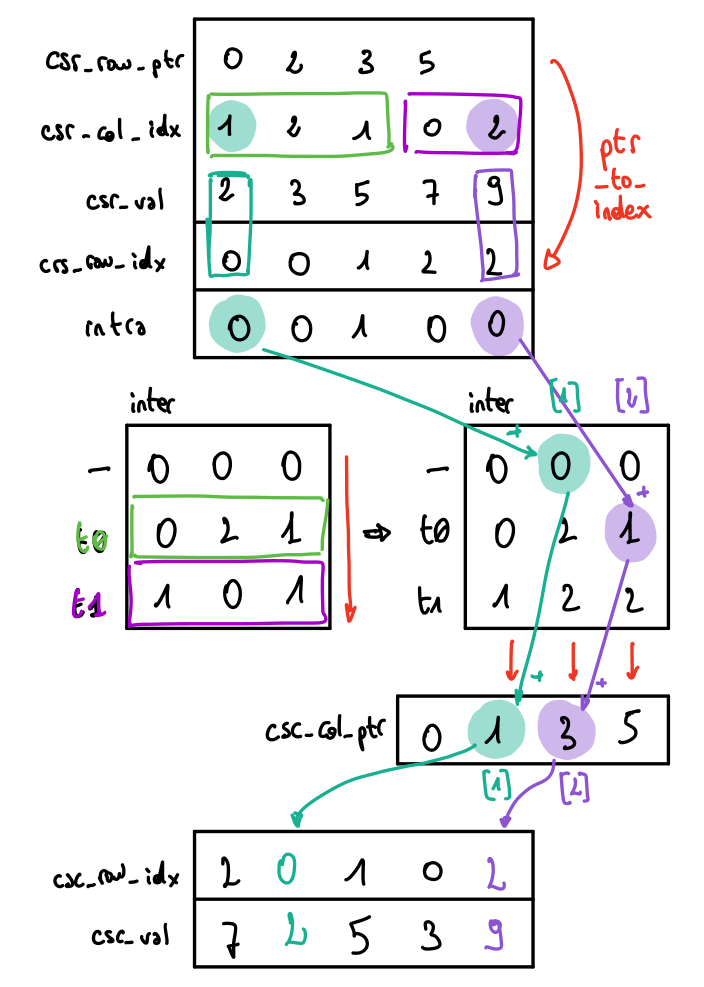
\includegraphics[scale=0.3]{transpose_scantrans.png}
	\caption{Algoritmo \ScanTrans}
	\label{transpose_algo_scantrans}
\end{figure}

L'algoritmo si sviluppa nel seguente modo:
\begin{enumerate}
    \item il vettore \var{csr\_row\_ptr} viene espanso per ottenere il vettore \var{csr\_row\_idx} attraverso la procedura \emph{pointers-to-indexes} che effettua l'operazione inversa dell'\emph{istogramma}; \\
    ora la struttura (\var{csr\_row\_idx}, \var{csr\_col\_idx}, \var{csr\_val}) rappresenta la matrice in formato COO ordinato per righe;
    \item decidiamo un numero arbitrario di thread $K$ che lavoreranno ciascuna su blocchi di $K/\mathrm{nnz}$ elementi. Allochiamo una matrice $\var{inter}$ di dimensioni $(K+1) \times n$ ed un vettore $\var{intra}$ di dimensione $\mathrm{nnz}$. La prima manterrà nella $(i+1)$-esima riga l'istogramma parziale relativo all'$i$-esimo blocco. La seconda mantiene un offset di colonna di ciascun elemento;
    \item i $K$ thread eseguono l'\emph{istogramma} ciascuna sul proprio blocco, la matrice $\var{inter}$ viene riempita;
    \item viene applicata l'operazione \emph{scan} ad ogni colonna della matrice \var{inter};
    \item il vettore \var{csc\_col\_ptr} viene ottenuto copiando l'ultima riga di \var{inter} ed applicando al vettore risultante l'operazione \emph{scan};
    \item riordiniamo gli elementi nei vettori \var{csr\_row\_idx}, \var{csr\_val} ottenendo quindi \var{csc\_row\_idx}, \var{csc\_val}; \\
    la nuova posizione dell'elemento $i$-esimo viene calcolata nel seguente modo:
    \begin{itemize}
        \item $b = i / \mathrm{nnz}$;
        \item $c = \var{csc\_col\_idx}[i]$;
        \item $l = \var{csc\_col\_ptr}[c] + \var{inter}[b n + c] + \var{inter}[c]$;
        \item $\var{csc\_val}[l] \leftarrow \var{csr\_val}[j]$;
        \item $\var{csc\_row\_idx}[l] \leftarrow \var{csr\_row\_idx}[j]$.
    \end{itemize}
\end{enumerate}

Il funzionamento dell'algoritmo è illustrato in Figura~\ref{transpose_algo_scantrans}. 

\subsection{MergeTrans}

\begin{figure}[htbp]
    \centering
	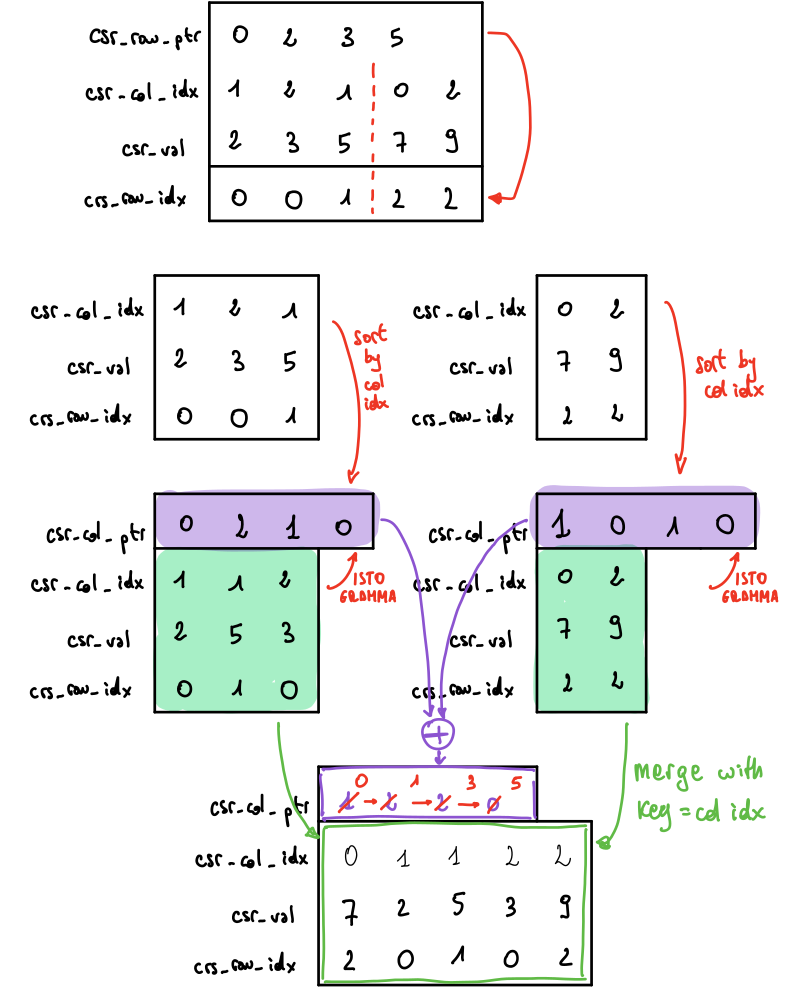
\includegraphics[scale=0.3]{transpose_mergetrans.png}
	\caption{Algoritmo \MergeTrans}
	\label{transpose_algo_mergerans}
\end{figure}
	
Il precedente algoritmo esegue nello step (6) un insieme di accessi casuali in memoria che non permettono di sfruttare in modo adeguato la shared memory. 

Per mitigare questo aspetto negativo viene introdotta una variante di questo algoritmo che, se implementato correttamente, permette ai thread di lavorare sempre con un numero costante, contiguo di elementi. 
	
L'algoritmo considerato prevede due passi importanti: \textit{sort} e \textit{merge}.

Inizialmente sono stati creati gli indici di riga a partire dai puntatori delle colonne e su questi ultimi è stato fatto un sort su piccole porzioni di array, mantenendo quindi i vari blocchi disordinati tra di loro ma con gli elementi ordinati. 

Successivamente è stato utilizzato il merge ricorsivo partendo dai blocchi più piccoli e unendoli in blocchi sempre più grandi. Per funzionare questo processo necessita dell'utilizzo di due buffer di memoria che contengono gli elementi appena ordinati. 

Infine dai puntatori delle colonne vengono estraxtti gli indici e viene fatta la scan che ritorna il risultato in formato \textit{csc}.

Il funzionamento dell'algoritmo è illustrato in Figura~\ref{transpose_algo_mergerans}. 

%\begin{figure}[H]
%	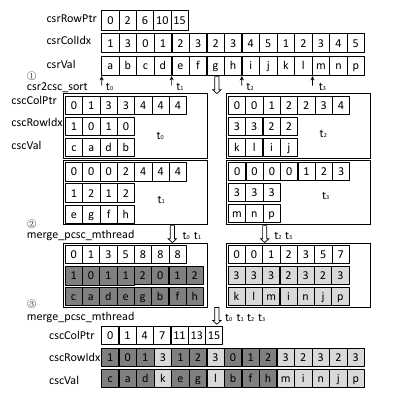
\includegraphics[scale=0.6]{mergetrans.png}
%	\caption{Merge Trans, esempio utilizzato in \cite{parallelTrans}.}
%	\label{mergetrans}
%\end{figure}

\subsection{NVidia cuSPARSE}

I risultati temporali di tutti gli algoritmi precedentemente descritti saranno confrontati con l'implementazione di NVidia della trasposta della matrice sparsa. 

La libreria \cuSPARSE{} è parte di \textrm{CUDA Toolkit}, insieme di librerie utilizzate per effettuare operazioni tra vettori e matrici attraverso diversi formati. 

Versioni diverse di \textrm{CUDA Toolkit} implementano funzioni con nomi diversi e funzionamenti diversi. In particolare per \textrm{Cuda Toolkit 9.0} possiamo trasporre la matrice sparsa attraverso la procedura \texttt{cusparseScsr2csc}.

Nella versione \textrm{Cuda Toolkit 10.2} viene esposto il metodo \texttt{cusparseCsr2cscEx2} che effettua la trasposta in due possibili modi a seconda se il parametro ``algoritmo" è valorizzato con la costante \texttt{CUSPARSE\_CSR2CSC\_ALG1} oppure \texttt{CUSPARSE\_CSR2CSC\_ALG2}. Le due versioni differiscono per le tempistiche e per il consumo di memoria (maggior memoria necessaria per la seconda implementazione). Le tempistiche sono riportate in Tabella~\ref{results}.

La libreria è dettagliatamente documentata in \cite{cusparse}. A seconda della versione di \emph{CUDA} dobbiamo modificare lo script di compilazione. In particolare il \emph{Makefile} del progetto permette di compilare per due architetture specifiche, una con CUDA 9 e l'altra CUDA 10/11. 